%general
Am 17. Oktober 2013 war der Startschuss der Veranstaltung. Die ersten Termine waren im Sinne der Wissensreaktivierung gestaltet. In mehreren Terminen wurden die grundlegenden Konzepte von Rechnerarchitekturen wiederholt, um Wissenslücken zu schließen und alle auf einen Stand zu bringen. Erst später ging die eigentliche Projektphase los.

Nach den Vorlesungsterminen ging es in die Gruppen. Jede Gruppe bestand aus 5-8 Personen. Unsere Gruppe bestand aus 5 Leuten und war damit die Kleinste. Ab diesem Zeitpunkt waren die Gruppen auf sich gestellt. Die Lehrkräfte waren nicht mehr für die Organisation zuständig, sondern hatten nur noch unterstützende und beratende Aufgaben.

In den ersten Wochen wurde noch nicht so viel Praktisches gemacht. Wir teilten uns zunächst in eine Hardware- und Softwaregruppe auf. Damit beide Teilgruppen an einem Strang ziehen, investierten wir die Zeit in den ersten Wochen für eine kleine Ideensammlung bezüglich unserer ISA und unserer Befehlsstruktur. Es wurden Fragen grundlegende Fragen geklärt wie z.B. die Wort- und Adressbreite, Little oder Big Endian und wie unsere Befehlsstruktur aufgebaut ist. Ein Teil unserer Ideensammlung der ersten Wochen ist in der Abbildung „Ideensammlung“ zu sehen.

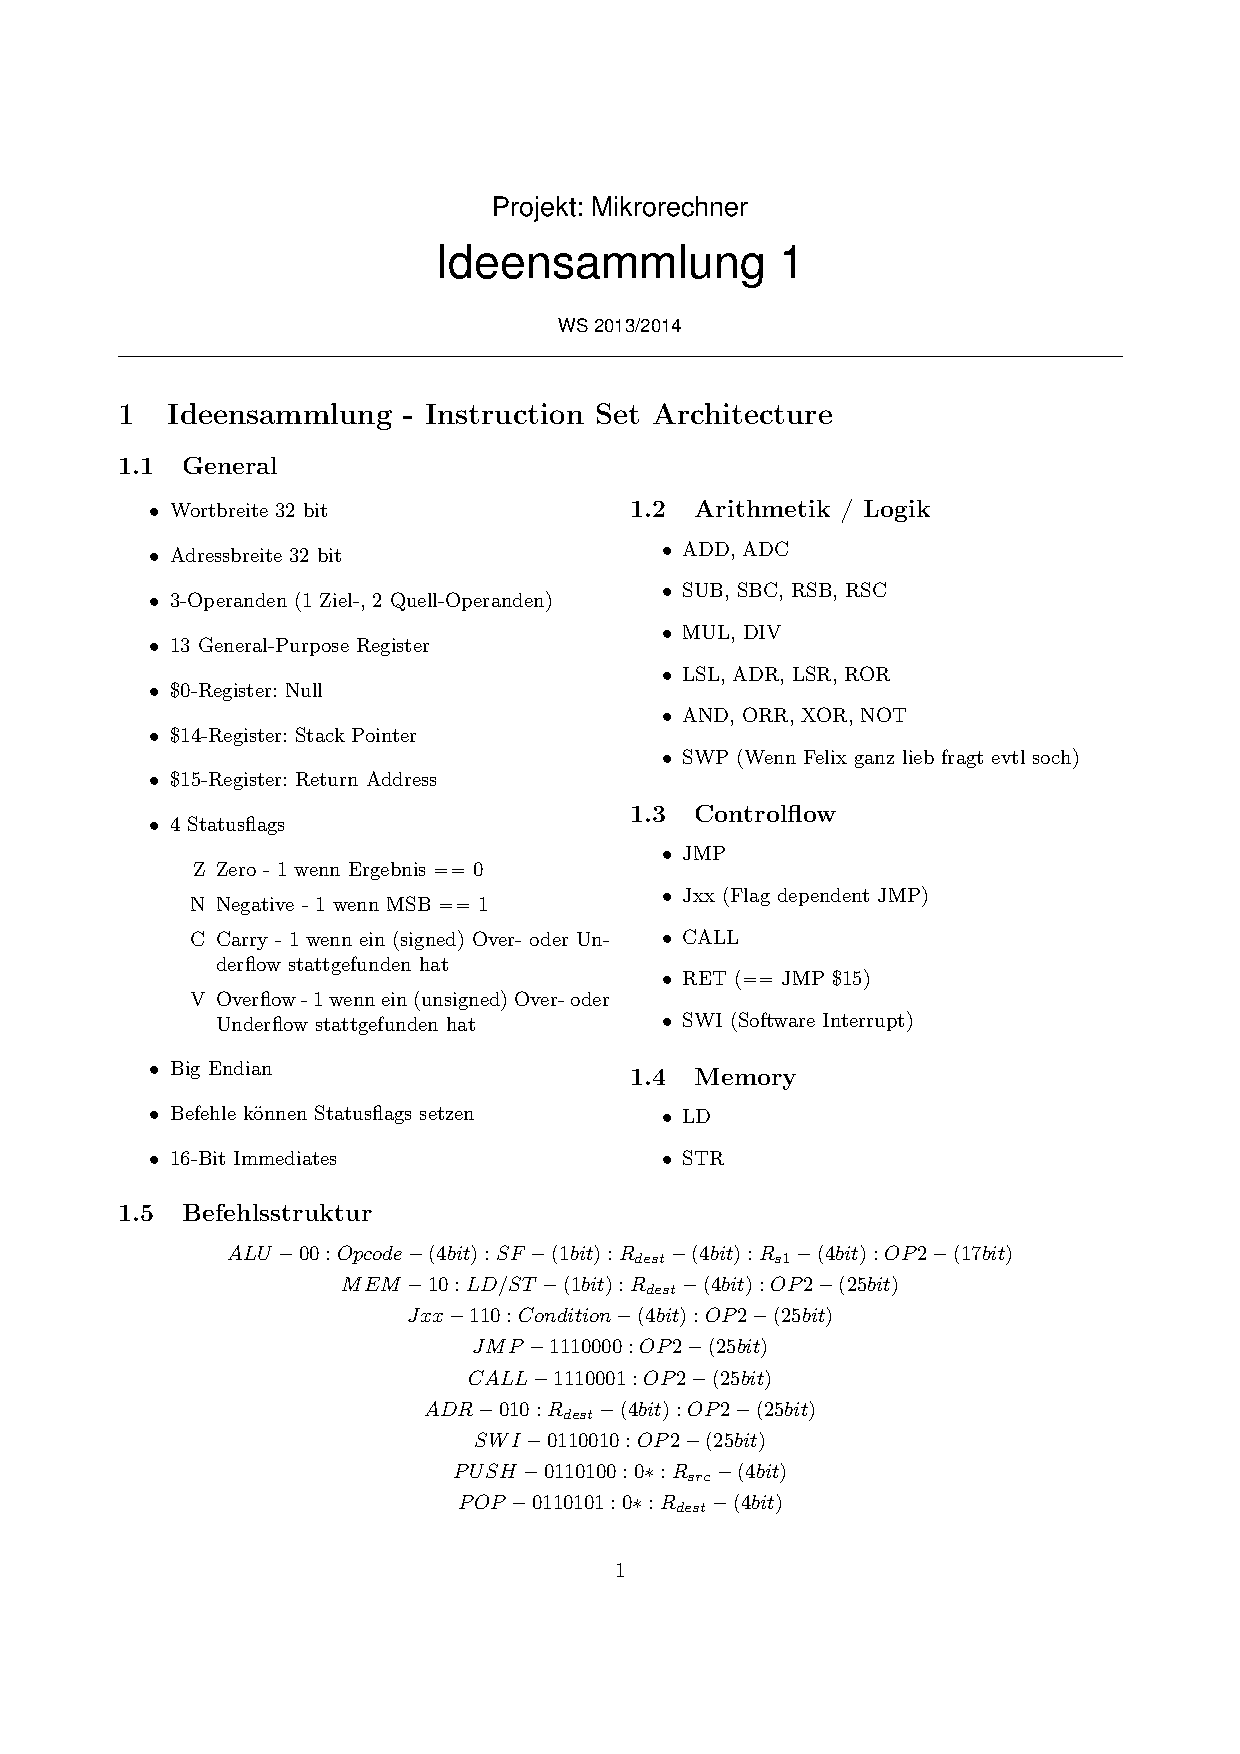
\includegraphics{images/Ideensammlung}

 Um eine gute Kommunikation zu gewährleisten, trafen wir uns jeden Donnerstag am Informatikum. Wir arbeiteten alle in einem Raum, weil uns eine direkte Kommunikation wichtig war. Bei Problemen konnte so der direkte Kontakt hergestellt werden. Denn es stellte sich schnell raus, dass Abweichungen von der ersten Ideensammlung unumgänglich waren. So konnten Konflikte schnell diskutiert und beseitigt werden.

Darüber hinaus nutzten wir Git, um die Ergebnisse zusammenzutragen und alle auf einem Stand zu halten. Außerdem konnten so Fragen sofort geklärt werden und mussten nicht bis auf den nächsten Donnerstag verschoben werden.


\section{vorgehensweise inkl organisation}
% aufteilung in versch. gruppen
% treffen
% ticket systems, verwaltung von code, issue tracker
\section{warum python} %Ortmann
% weil myhdl (dazu kann marcel noch was sagen)
% und der rest ergab sich einfach
\section{ein wort zur lizenz} %Ortmann
% GPLv3
\section{tools}
\subsection{python}
\subsection{git}
\subsection{pycharm}
\subsection{latex}
\subsection{altera}
\subsection{hades}
\subsection{gtkwave}
\section{testen}
% unit testing



